\section{L"osungsansatz}
\rhead{L"osungsansatz}
\subsection{Diskretisation der R"uckprojektion}

Um nun dieses Problem zu l"osen m"ussen wir zuerst die Formel f"ur die
R"ucktransformation in eine riemannsche Summe umwandeln. So kann dann
das Integral durch Iteration von einfachen Additionen gel"ost werden.

R"uckprojektion:
\begin{equation}
	Bg(x,y) = \cfrac{1}{\pi}\int\limits_0^\pi g(x\cos{\vartheta}+y\sin{\vartheta},\vartheta) d\vartheta
\end{equation}\\
Angen"ahrt als Summe, erh"alt man:
\begin{equation}
	Bg(x,y) \approx \cfrac{1}{\pi}\sum_{i=1}^{n} g(\:\underbrace{x\cos{\vartheta_i}+y\sin{\vartheta_i}}_{\text{Radius}}\:,\!\underbrace{\vartheta_i}_\text{{Winkel}}\!) \Delta\vartheta
\end{equation}

\subsection{Beispiel einer R"uckprojektion}

Nun muss f"ur jeden Punkt der R"uckprojektion(c) diese Summe berechnet
werden. Der Winkel wird von 0 bis $\pi$ durchiteriert und f"ur jeden
Winkel, der sich an den errechneten Koordinaten der Radontransformation(b)
befindet, wird der Wert aufsummiert.

Das Inputbild ist das radontransformierte Orginalbild(a) es enth"alt
alle diskreten Werte der Funktion $g(r,\vartheta)$ welche der
Radontransformation entspricht.

\begin{figure}[ht!]\centering
	\subfigure[Orginalbild]{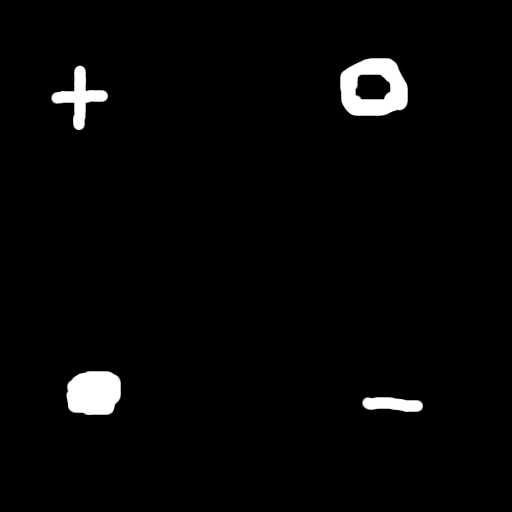
\includegraphics[width=0.3\textwidth]{radon/images/test.jpg}}
    \subfigure[Radontransformation]{
\includegraphics[width=0.3\textwidth]{radon/images/testTF.jpg}}
    \subfigure[R"uckprojektion]{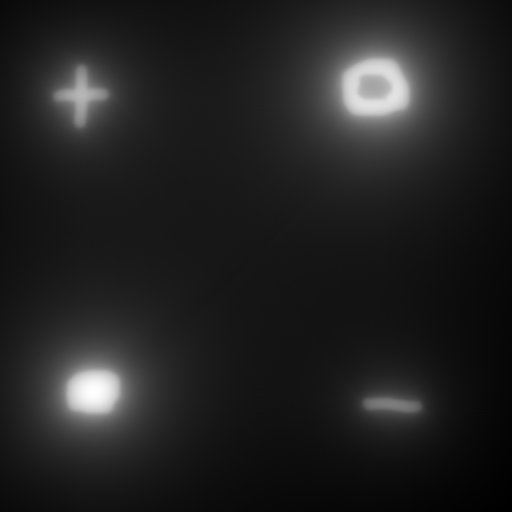
\includegraphics[width=0.3\textwidth]{radon/images/testBTF.jpg}}
\caption{Input und Output der R"uckprojektion}
\end{figure}
\FloatBarrier
